\documentclass{article}
\usepackage{pythonhighlight}
\usepackage{graphicx}
\usepackage{ctex}
\usepackage[left=3cm,top=3cm,right=3cm]{geometry}
\usepackage{hyperref}
% TITLE PAGE CONTENT %%%%%%%%%%%%%%%%%%%%%%%%
%%%%%%%%%%%%%%%%%%%%%%%%%%%%%%%%%%%%%%%%%%%%%
\newcommand{\labno}{08}
\newcommand{\labtitle}{EE208 Hadoop}
\newcommand{\authorname}{周李韬}
\newcommand{\studentno}{518030910407}
\newcommand{\classno}{F1803016}
% END TITLE PAGE CONTENT %%%%%%%%%%%%%%%%%%%%


\begin{document}

\begin{center}
{\LARGE \textsc{Laboratory No. \labno:} \\ \vspace{4pt}}
{\Large \textsc{\labtitle} \\ \vspace{4pt}} 
\rule[13pt]{\textwidth}{1pt} \\ \vspace{15pt}
{\large By: \authorname \\ \vspace{10pt}
No. \studentno \\ \vspace{10pt}
SJTU \classno \\ \vspace{10pt}
\today \vspace{20pt}}
\end{center}



\section{实验准备}

\subsection{实验环境}
\begin{itemize}
\item\textbf{Environment} Ubuntu 16.04 (on Virtual Machine)
\item\textbf{Tools} Hadoop 2.7.3, openjdk-8-jdk
\end{itemize}

\subsection{实验目的}

本实验中,我们需要安装、配置Hadoop,并完成一个分布式计算$\pi$的小练习。

\subsection{实验原理}
我们主要利用Hadoop中的mapreduce模型实现分布式计算,MAP步骤对原数据进行一次运算,每一条数据都会产生一至多个中间变量作为输出。在MAP步骤执行完毕后,中间变量会通过REDUCE函数进行结合、运算,通常情况下会返回与输入数据量相同的输出值。MAP-REDUCE的过程中,实际是将函数运算的结果存储了下来,而使得原本对相互关联的数据进行的运算得以被拆分成能够参与分布式运算的MAP、REDUCE过程,从而提升运算的效率。

本实验中,$\pi$的计算使用了向一个正方形进行随机投掷试验的方法,通过大量试验统计投掷结果位于正方形内接圆的概率,从而估算$pi$的值。通过几何概率模型,我们有
$$\frac{\mbox{投掷结果在圆中次数}}{\mbox{总投掷数}}=\frac{S_{\mbox{圆}}}{S_{\mbox{正方形}}} = \frac{\pi r^2}{(2r)^2} = \frac{1}{4}\pi$$
因此,我们只需编写程序模拟该过程,就可以得到$\pi$的估计值。

Hadoop Example中,使用了Halton Sequence生成随机数列,尽管通过该原理产生的数列是确定的,但当数列长度很大时,该随机数列的分布是均匀的,因此我们可以认为随着投掷次数增大,我们的试验结果会越来越趋向于$\pi$的理论值。

注意到我们在判断随机生成的点$(x,y)$是否位于圆中时,会计算$\sqrt{x^2+y^2}$与半径比较,该计算的时间较长,可以通过分布式计算降低运行时间。Hadoop Example中,将取点、判断的过程写入map函数,最后再通过reduce函数统计、估算$\pi$,实现分布式估计$\pi$的运算。

\section{实验步骤}

\subsection{安装Hadoop}

根据实验材料中的提示,我们在Linux虚拟机中为分配了账户,依次下载、安装了java8,Hadoop2.7.3,并完成了Hadoop的配置。

\subsection{计算$\pi$}

Hadoop计算$\pi$的原理已在上一节中进行解释。Hadoop Example中已对改运算进行了封装,我们调用时需要传入两个参数,map是运行map任务的个数,sample是每个map任务中取样的个数。map与sample之积就是一次统计中的全部试验个数。我们在命令行中调用该函数的命令如下。
\begin{python}
hadoopjar /usr/local/hadoop/share/hadoop/mapreduce/hadoop-mapreduce-examples-2.7.3.jar pi 2 10
\end{python}

试验结果如下所示:
\begin{table}[htbp]
\begin{tabular}{cccccc}
\hline
\textbf{Experiment} & \textbf{\begin{tabular}[c]{@{}c@{}}Number of\\ Maps\end{tabular}} & \textbf{\begin{tabular}[c]{@{}c@{}}Number of\\ Samples\end{tabular}} & \textbf{\begin{tabular}[c]{@{}c@{}}Total Sample\\ Counts\end{tabular}} & \textbf{\begin{tabular}[c]{@{}c@{}}Running\\ Time(s)\end{tabular}} & \textbf{\begin{tabular}[c]{@{}c@{}}Estimated\\ pi\end{tabular}} \\ \hline
1                   & 2                                                                 & 10                                                                   & 20                                                                     & 18.275                                                             & 3.8                                                             \\
2                   & 5                                                                 & 10                                                                   & 50                                                                     & 22.300                                                             & 3.28                                                            \\
3                   & 1                                                                 & 100                                                                  & 100                                                                    & 17.244                                                             & 3.2                                                             \\
4                   & 10                                                                & 10                                                                   & 100                                                                    & 26.427                                                             & 3.2                                                             \\
5                   & 2                                                                 & 100                                                                  & 200                                                                    & 17.759                                                             & 3.12                                                            \\
6                   & 10                                                                & 100                                                                  & 1000                                                                   & 27.978                                                             & 3.148                                                           \\
7                   & 20                                                                & 100000                                                               & 2000000                                                                & 48.594                                                             & 3.141504                                                        \\
8                   & 100                                                               & 100000                                                               & 10000000                                                               & 75.672                                                             & 3.1415844                                                       \\
9                   & 10                                                                & 1000000                                                              & 10000000                                                               & 27.616                                                             & 3.1415844                                                       \\
10                  & 10                                                                & 10000000                                                             & 100000000                                                              & 27.340                                                             & 3.14159256                                                      \\ \hline
\end{tabular}
\end{table}

从相同样本数的实验中可以得知,在不改变随机数列的种子的情况下,该样例的算法是确定性的。比较3、4实验可得,在数据量较小的情况下,Maps过多会增加运行时间,比较8、9实验可得,过多的Maps在超过本机运行能力的情况下,也会拖慢运行时间,比较9、10实验则可得,在选取合适的Maps条件下,分布式计算能够有效减小甚至消除由于样本数增多而造成的时间消耗。根据实验结果所得,当样本数达到$10^8$数量级时,$\pi$的估算能够达到5位小数的精度。


\begin{figure}[htbp]
\centering
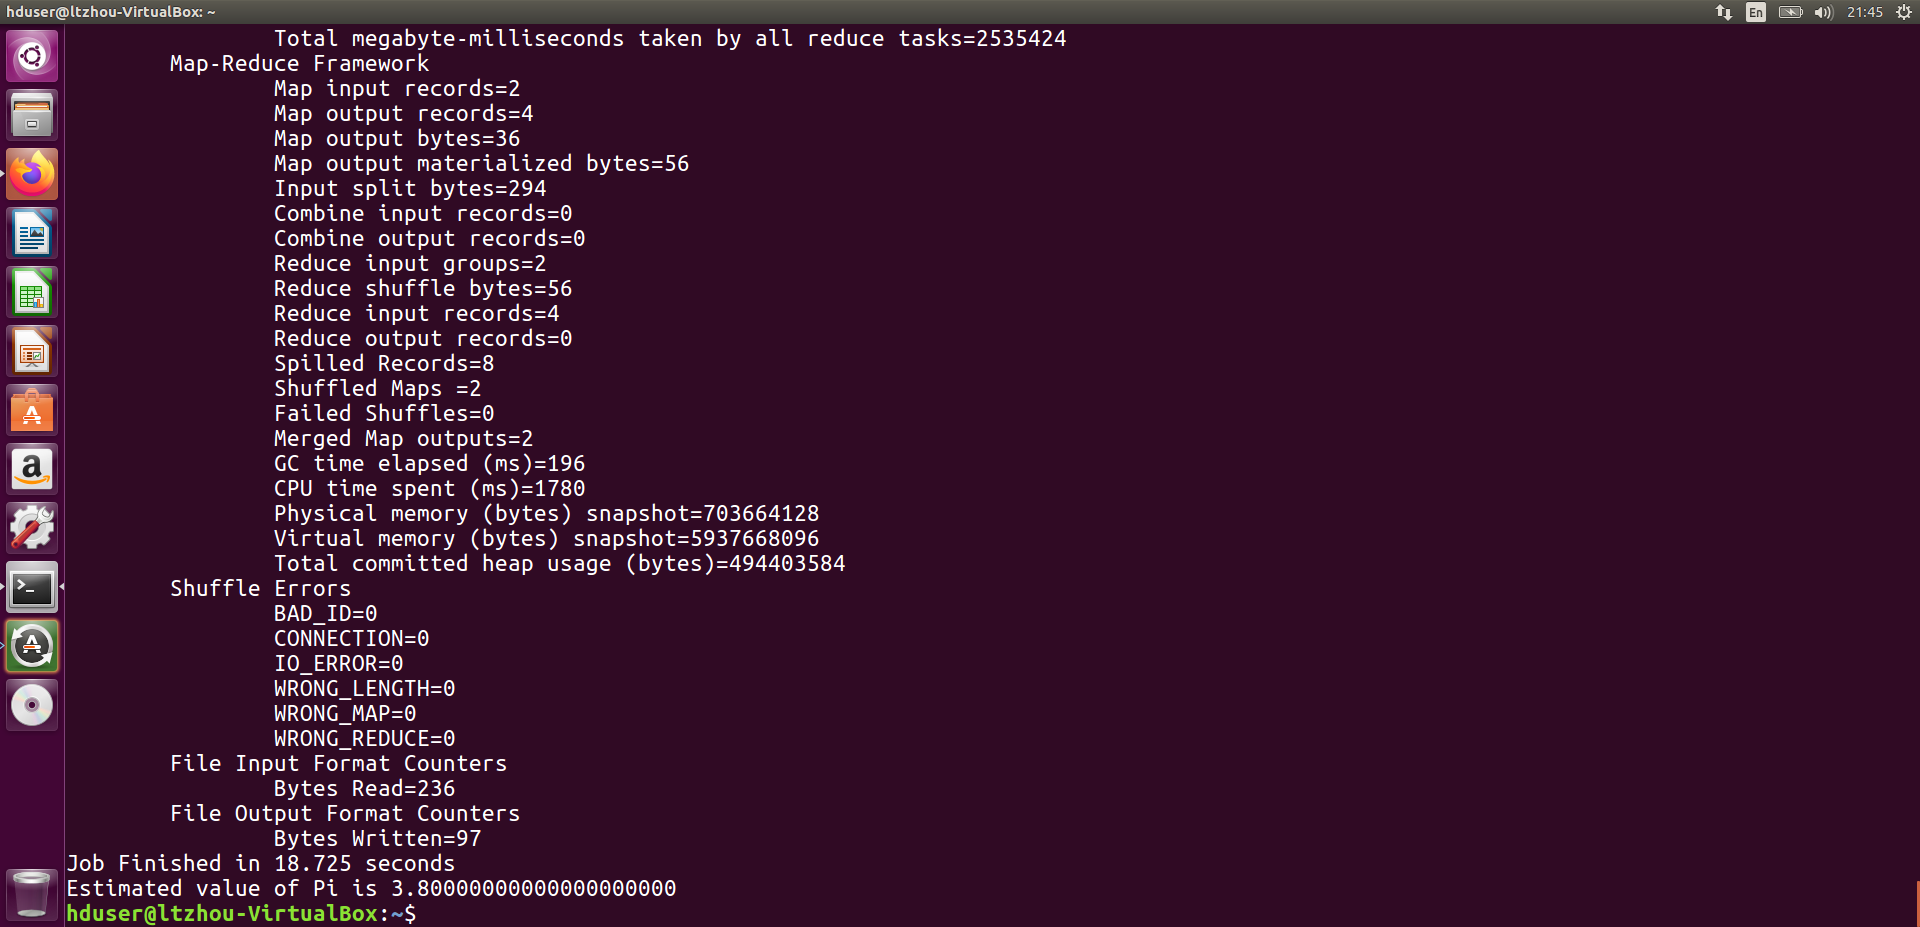
\includegraphics[width=13.5cm]{img/2-10.png}
\caption{Map=2, Sample=10时运行结果实例}
\label{fig:2-10}
\end{figure}

\begin{figure}[htbp]
\centering
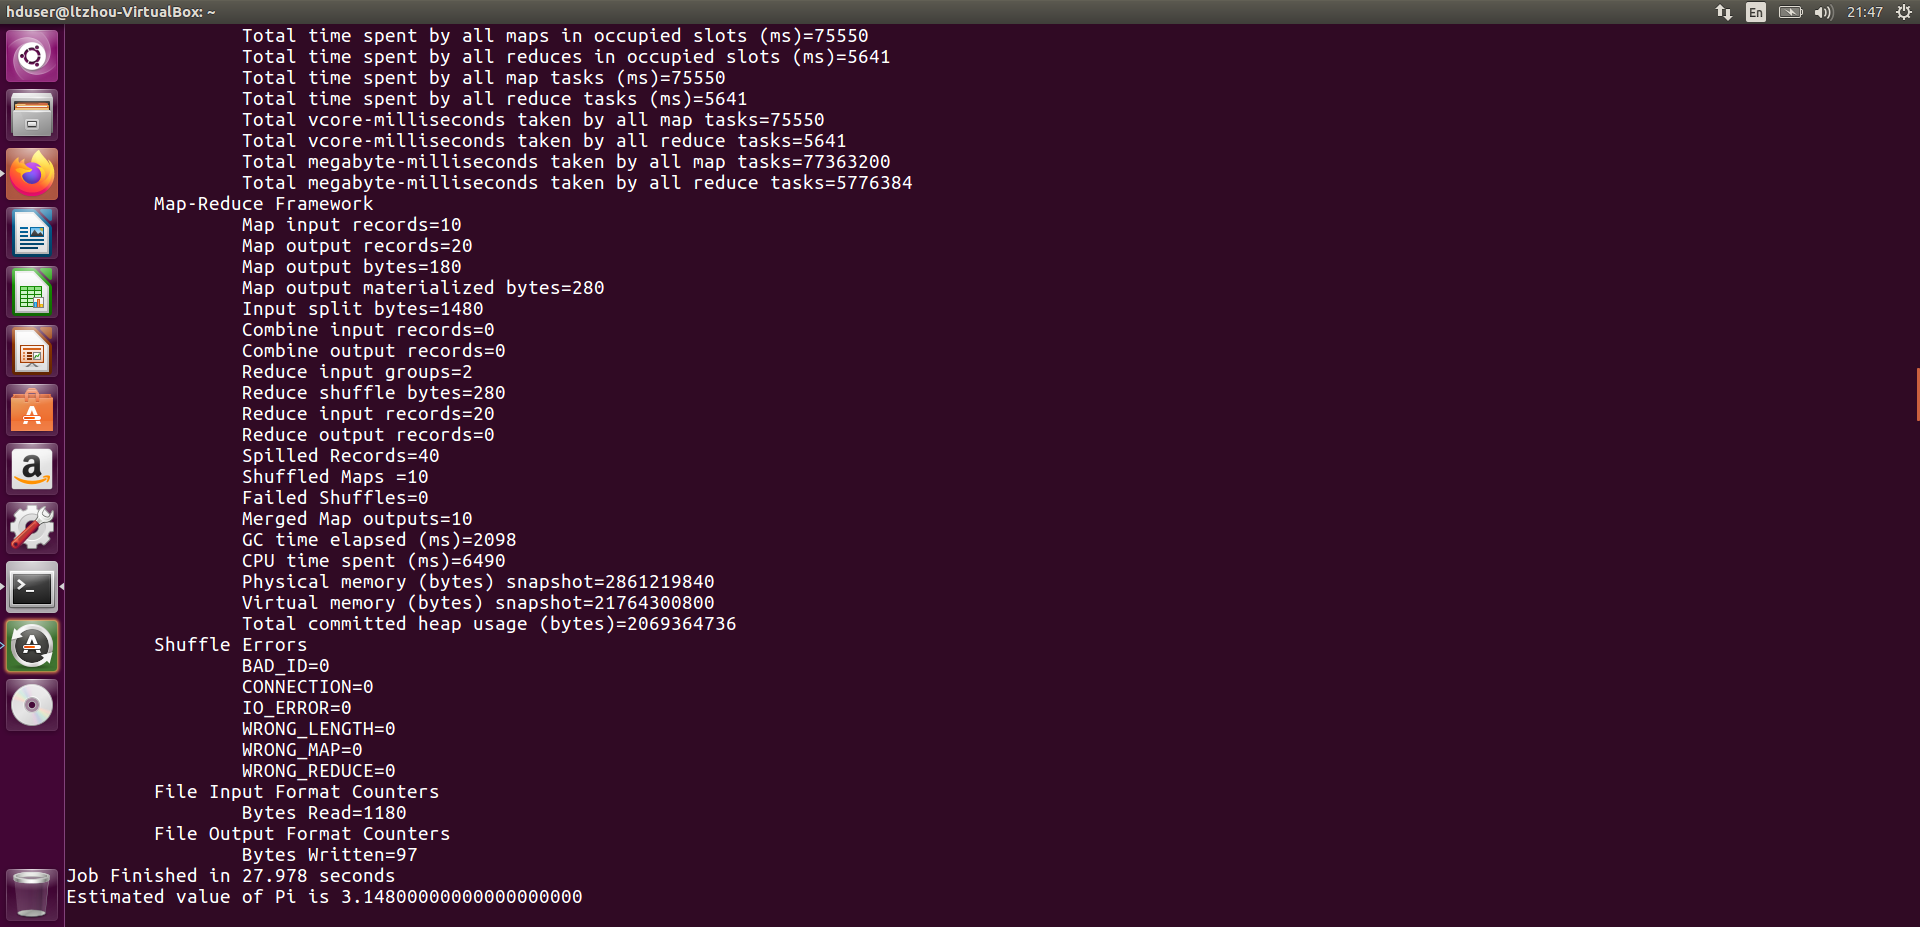
\includegraphics[width=13.5cm]{img/10-100.png}
\caption{Map=10, Sample=100时运行结果实例}
\label{fig:2-10}
\end{figure}



\section{实验总结}
\paragraph{概述}
本实验中,我们完成了Hadoop的安装、配置,并通过实验分布式地计算了$\pi$的估计值。

\paragraph{感想}
通过本次实验的学习,我体会到到了分布式运算带来的运算效率提升。分布式运算能够帮助我们更充分地利用、扩展现有的硬件资源,带来性能的提升。我也通过实验的尝试,学习了MAP-REDUCE模型的思想,希望这次实验的学习能够为以后的LAB做好铺垫。


\end{document}

